\subsection{Particle and pair selection}
\label{sec:ParticlePairSelection}


\subsubsection{\texorpdfstring{$\Lambda$}{Lambda} reconstruction}
%\subsubsection{$\Lambda$ reconstruction}
\label{sec:Recon}

$\Lambda$ are neutral particles, and as such we do not directly detect them.  
Instead, $\Lambda$ are topologically reconstructed by looking for the daughter tracks that they decay into.  
The general term for particles reconstructed this way (including $\bar{\Lambda}$ and $K^0_\mathrm{s}$) is V0.

For each event, the list of AliAODv0 objects is used as an initial list of V0 candidates.  
Only AliAODv0 objects with (AliAODv0::GetOnFlyStatus() == false) are used.  
These are V0s constructed offline by the AliV0Vertexer using combined TPC-ITS tracking (or TPC-only if the ITS is inactive).  
After obtaining a list of V0 candidates, the following cuts were applied for each V0's daughter tracks.

\begin{itemize}
\item The V0 was rejected if (AliAODv0::GetNDaughters() $> 2$), and the daughters are required to have different charges.
\item The daughter tracks were required to have hits on at least 80 pad rows of the TPC.
\item The daughter protons (antiprotons) were required to have $p_{\rm T} > 0.5 (0.3)$ GeV/c, and the daughter pions required $p_{\rm T} \geq 0.16$ GeV/c. 
The difference between proton and antiproton $p_{\rm T}$ cuts arises from a need to minimize contaminations from material protons. 
All daughters were required to be in the range $|\eta| < 0.8$.
\item The TPC was used for PID purposes.  
A daughter was considered a proton and/or pion if the PID resolution task returned a respective $\mathrm{d}E/\mathrm{d}x$ NSigma value less than 3 for it.
\item Daughter tracks were required to have a TOF PID NSigma value less than 4 if the TOF signal was available.
\item The two daughters are required to have a AliAODv0::DcaV0Daughters() $< 0.4$ (the vertexer computes this DCA using resolution weighting, so the units here should probably be called "effective cm").
\item The proton daughter was required to have a DCA to the primary vertex $> 0.1$ cm.
\item The pion daughter was required to have a DCA to the primary vertex $> 0.3$ cm.
\end{itemize}

Each V0 is then subjected to the following cuts:
\begin{itemize}
\item The V0 is required to have $|\eta| < 0.8$.
\item The V0 is required to have a proper decay length less than 60 cm.
\item The cosine of the pointing angle must be greater than 0.9993.
\item The DCA of the V0 to the primary vertex must be less than 0.5 cm.
\item For a $\Lambda$ was required to have a proton daughter and a $\pi^-$ daughter (as determined using the above PID cuts).  
For a $\bar{\Lambda}$, an antiproton and $\pi^+$ daughter were required.
\item For both $\Lambda$ and $\bar{\Lambda}$, the reconstructed invariant mass was required to fall within $\abs{m_\mathrm{inv}-m_\mathrm{PDG}} < 3.8$ MeV.  
Note that this cut value was determined by inspection of the $p_\mathrm{T}$-integrated invariant mass peak.  
Future investigation of $p_\mathrm{T}$-dependent invariant mass peak and subsequently enforcing a $p_\mathrm{T}$-dependent cut could lead to better background reduction.  
Also, close inspection of Figure \ref{fig:BothInvMass} shows that the peak multiplicity occurs at a mass slightly higher (several tenths of an MeV) than the PDG mass value.  
As such, it may be better to use an invariant mass window centered around the reconstructed peak value, rather than the PDG mass.  
This will also be investigated in the future.
\end{itemize}

The optimal cut values were determined by comparing distributions of reconstructed $\Lambda$ in Monte Carlo HIJING events with simulated detector effects.  
The data set (LHC12a17a\_fix) included injected strange signals (extra $\Lambda$, $\bar{\Lambda}$, $\Xi$, and $\Omega$ in each event).  
Initially, V0s were reconstructed without distinguishing between injected signals and particles from the underlying event.  
However, a disparity was seen between the average reconstruction efficiency of mulitistrange hyperons and antihyperons (see Sec.\ \ref{sec:InjectedMCSignals} for more details).  
The analysis was then performed with the injected signals removed, and the disparity went away.  A primary particle (AliAODMCParticle) was considered injected if it had AliAODMCParticle::GetLabel() greater than AliGenHijingEventHeader::NProduced()$-1$. 
Likewise, a secondary particle (e.g. $\Lambda$ resulting from decay of a $\Sigma$ baryon) was considered injected if it's mother particle had AliAODMCParticle::GetLabel() greater than AliGenHijingEventHeader::NProduced()$-1$.  
Subsequent Monte Carlo analyses have been performed with the injected signals removed.

$\Lambda$ were reconstructed and their corresponding AliAODMCParticle objects were consulted in order to classify the $\Lambda$ into different categories: Real, primary $\Lambda$; secondary $\Lambda$ coming from decays of $\Sigma$ (or $\Sigma$ excited states); secondary $\Lambda$ coming from decays of $\Xi$, $\Omega$, and other sources; fake $\Lambda$; and $K^0_\mathrm{s}$ that have been misidentified as $\Lambda$.  
For each cut parameter (e.g. cosine of pointing angle), a plot was made showing the distributions of V0 candidates of the various types.  
These plots contain only the parameter distributions of candidates that pass all the other cuts.  Figures \ref{fig:LambdaCutDists1} and \ref{fig:LambdaCutDists2} show these distributions for the different $\Lambda$ types.  
Figures \ref{fig:AntiLambdaCutDists1} and \ref{fig:AntiLambdaCutDists2} show the equivalent results for $\bar{\Lambda}$.

\begin{figure}
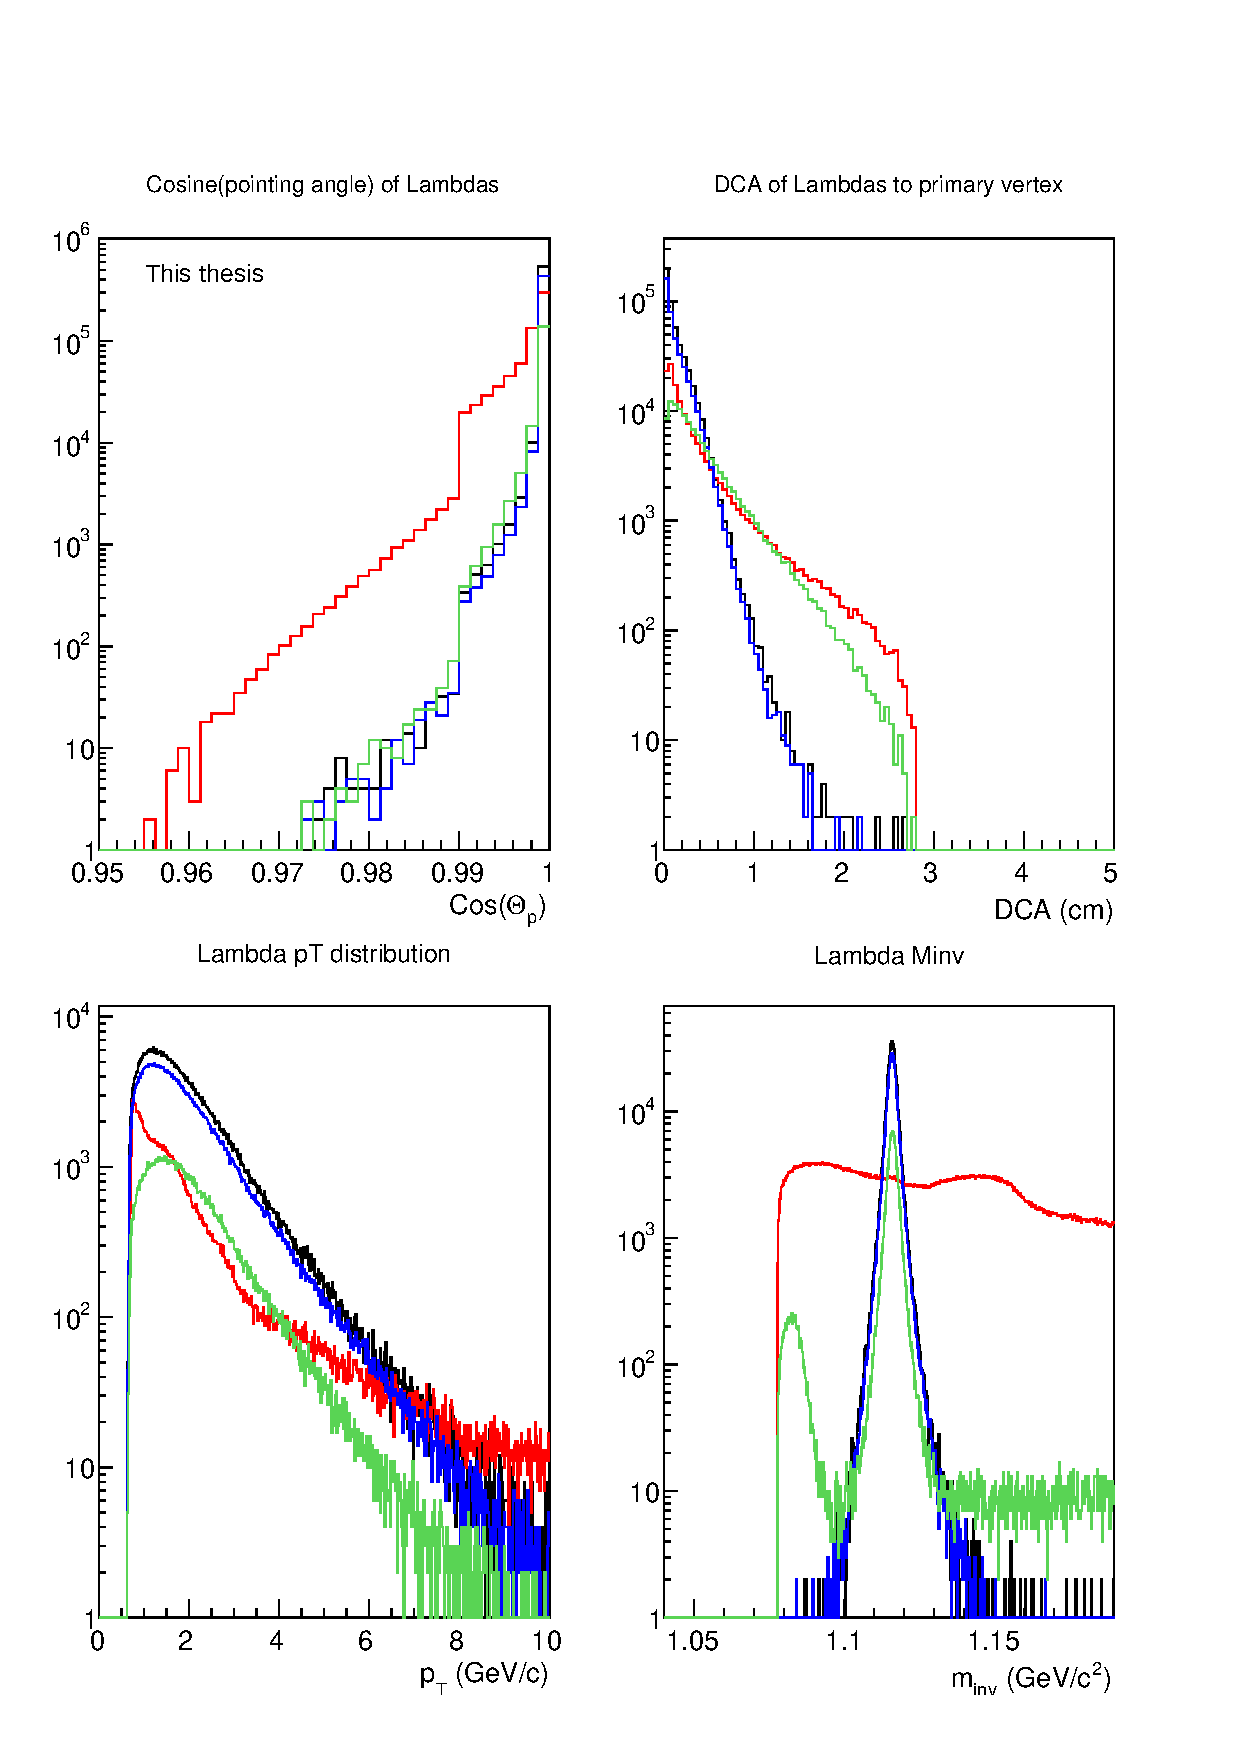
\includegraphics[width=36pc]{Figures/2014-03-31-Distribution-Lambda-4Types-CosP-DCA-pT-Minv.pdf}
\caption[$\Lambda$ cut distributions]{$\Lambda$ cut distributions shown for real $\Lambda$ (black), $\Lambda$ from $\Sigma$ decay (blue), secondary $\Lambda$ from other sources (green), fake $\Lambda$ (red). 
Optimal cut values were set such that a looser cut would differentially add more fake and (non-$\Sigma$) secondary $\Lambda$ than primary $\Lambda$}
\label{fig:LambdaCutDists1}
\end{figure}

\begin{figure}
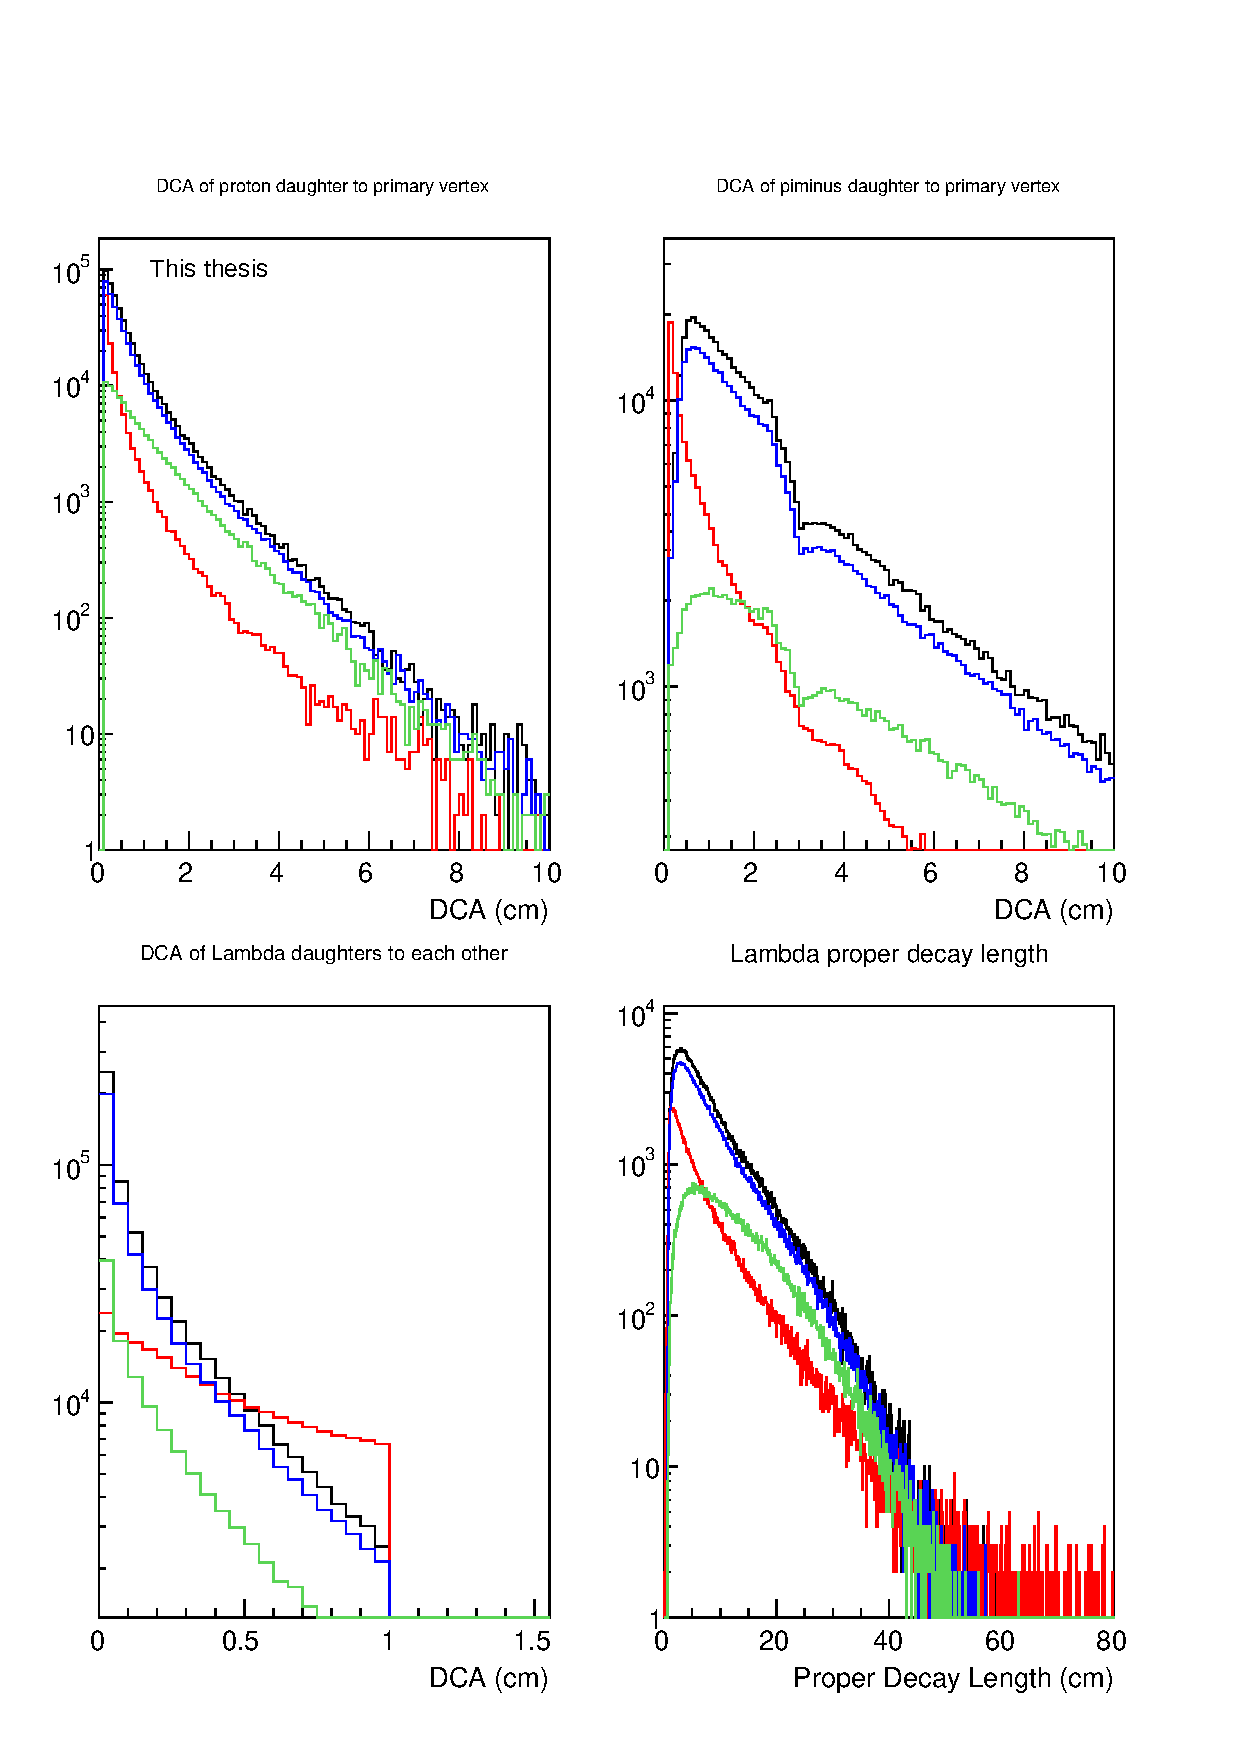
\includegraphics[width=36pc]{Figures/2014-03-31-Distribution-Lambda-4Types-DCA-DCA-DCA-DecayLength.pdf}
\caption[$\Lambda$ cut distributions]{$\Lambda$ cut distributions shown for real $\Lambda$ (black), $\Lambda$ from $\Sigma$ decay (blue), secondary $\Lambda$ from other sources (green), fake $\Lambda$ (red). 
Optimal cut values were set such that a looser cut would differentially add more fake and (non-$\Sigma$) secondary $\Lambda$ than primary $\Lambda$}
\label{fig:LambdaCutDists2}
\end{figure}

\begin{figure}
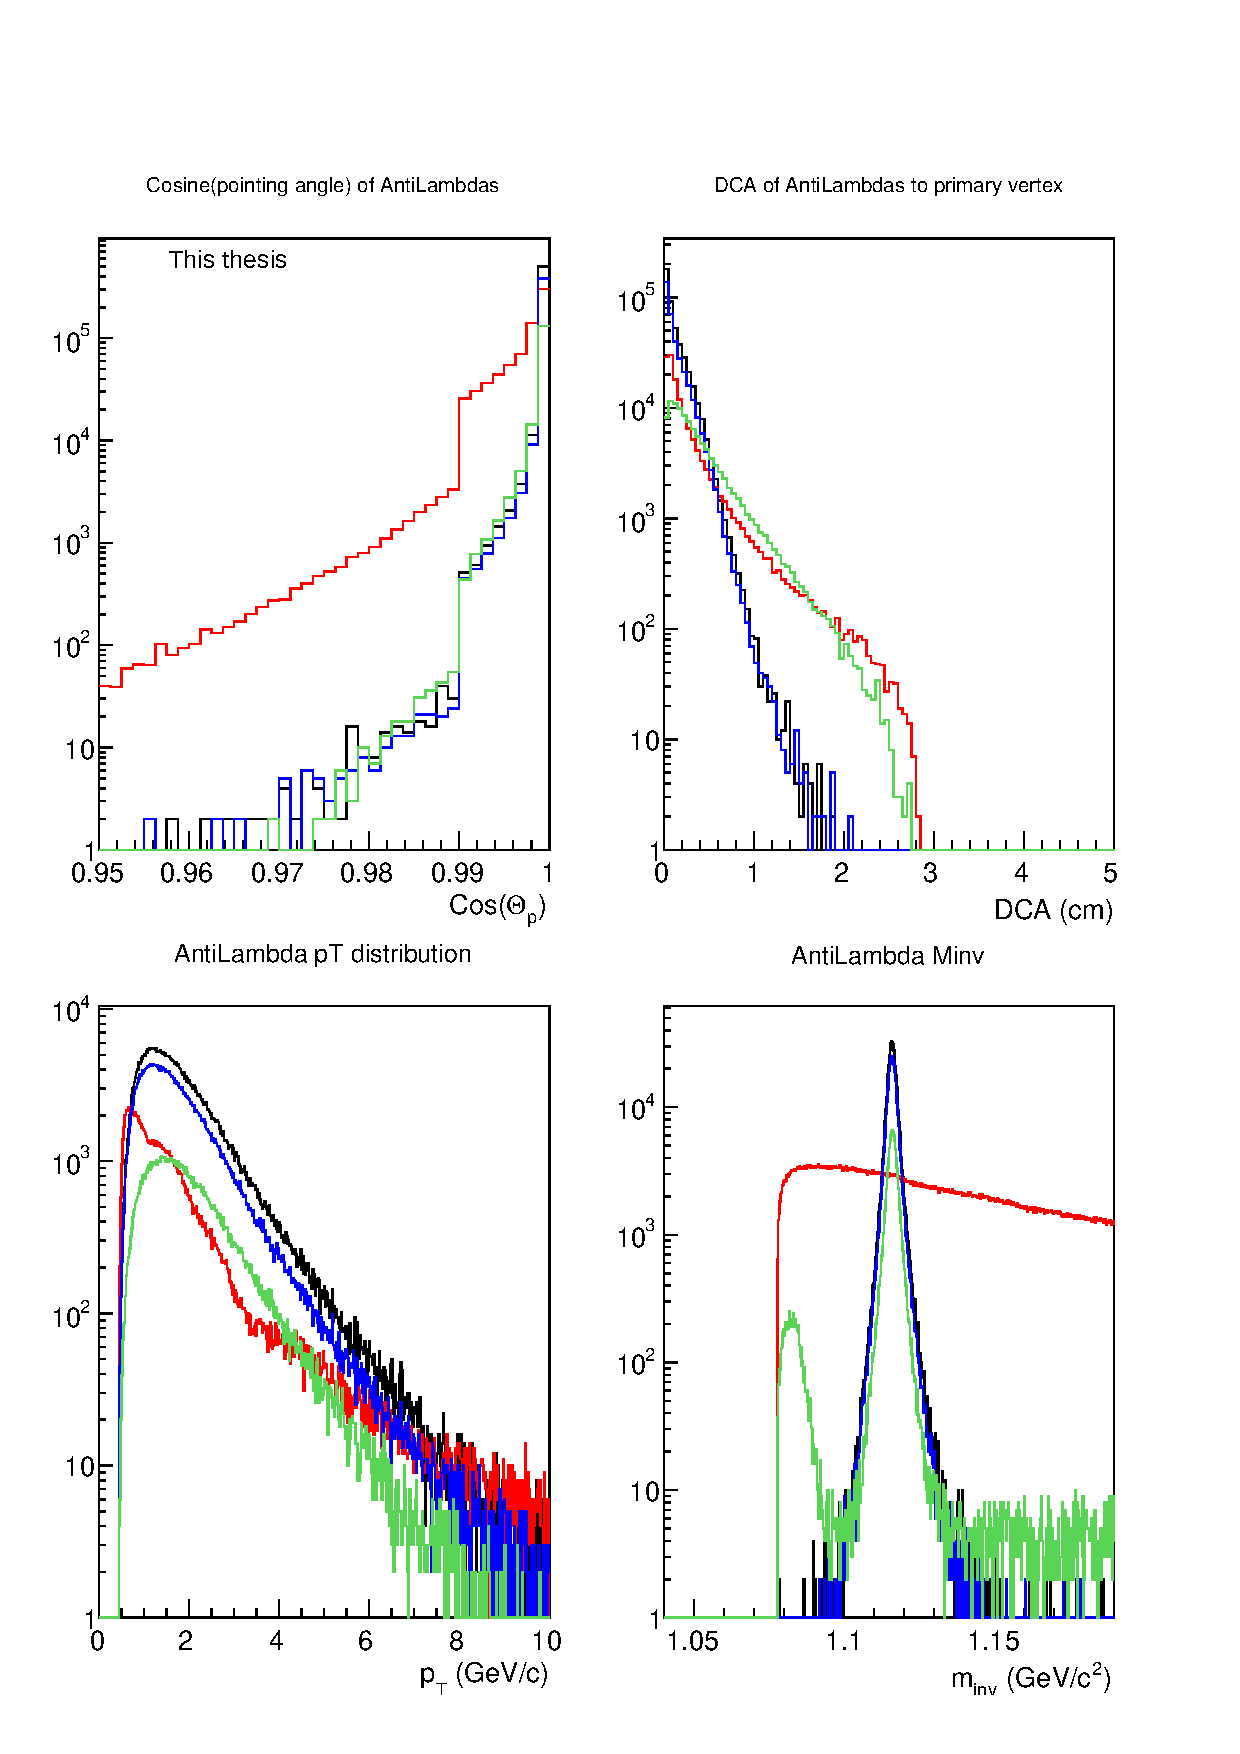
\includegraphics[width=36pc]{Figures/2014-03-31-Distribution-AntiLambda-4Types-CosP-DCA-pT-Minv.pdf}
\caption[$\bar{\Lambda}$ cut distributions]{$\bar{\Lambda}$ cut distributions shown for real $\bar{\Lambda}$ (black), $\bar{\Lambda}$ from $\Sigma$ decay (blue), secondary $\bar{\Lambda}$ from other sources (green), fake $\bar{\Lambda}$ (red). 
Optimal cut values were set such that a looser cut would differentially add more fake and (non-$\bar{\Sigma}$) secondary $\bar{\Lambda}$ than primary $\bar{\Lambda}$}
\label{fig:AntiLambdaCutDists1}
\end{figure}

\begin{figure}
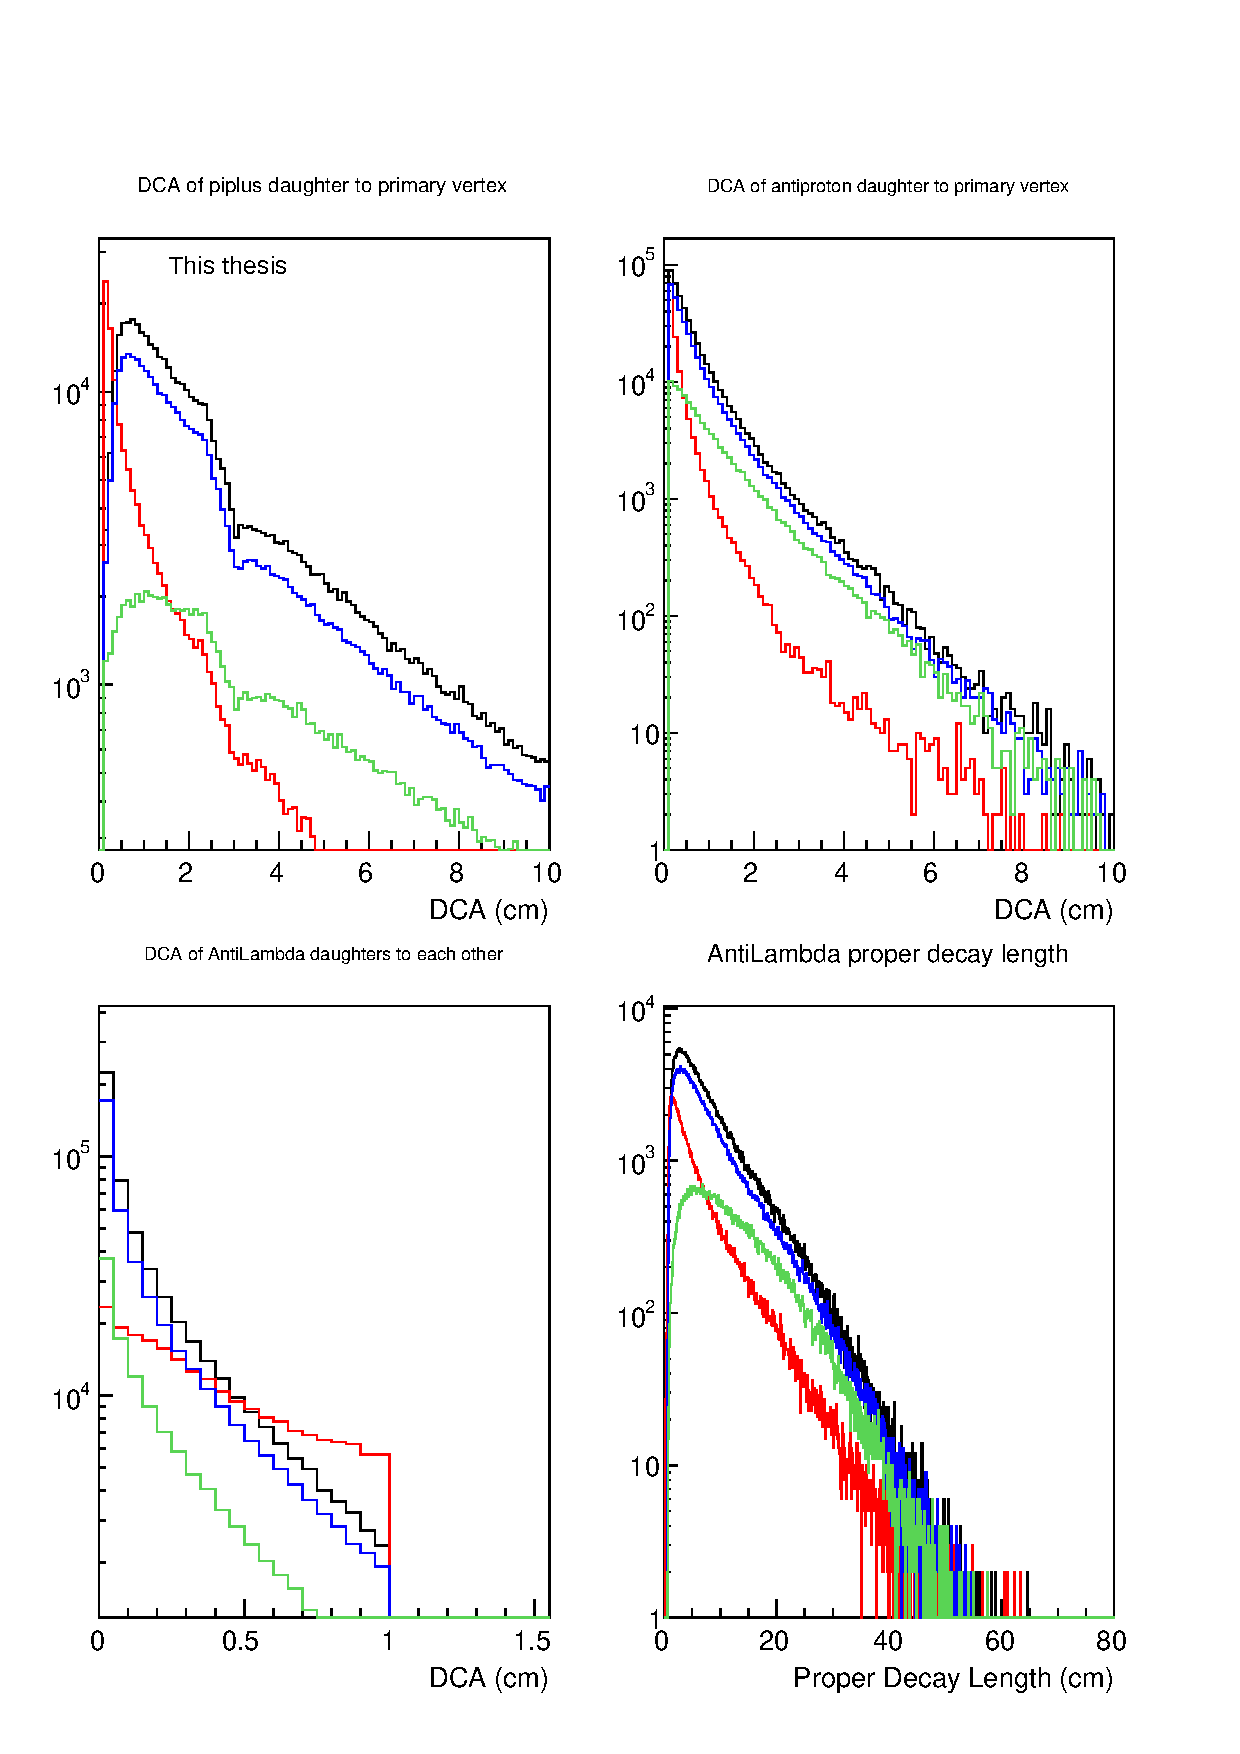
\includegraphics[width=36pc]{Figures/2014-03-31-Distribution-AntiLambda-4Types-DCA-DCA-DCA-DecayLength.pdf}
\caption[$\bar{\Lambda}$ cut distributions]{$\bar{\Lambda}$ cut distributions shown for real $\bar{\Lambda}$ (black), $\bar{\Lambda}$ from $\Sigma$ decay (blue), secondary $\bar{\Lambda}$ from other sources (green), fake $\bar{\Lambda}$ (red). 
Optimal cut values were set such that a looser cut would differentially add more fake and (non-$\bar{\Sigma}$) secondary $\bar{\Lambda}$ than primary $\bar{\Lambda}$}
\label{fig:AntiLambdaCutDists2}
\end{figure}

For the construction of Figures \ref{fig:LambdaCutDists1},\ref{fig:LambdaCutDists2},\ref{fig:AntiLambdaCutDists1}, and \ref{fig:AntiLambdaCutDists2}, each $\Lambda$ type was preselected using AliAODMCParticle information, and only V0 candidates of that type were reconstructed in that analysis run. 
This was done for ease of histogramming the distributions.  
Roughly equal numbers events were analyzed for each run type, with the exception of the analysis of the primary $\Lambda$.  That analysis run utilized only about half the data set.  
Therefore, the primary $\Lambda$ ($\bar{\Lambda}$) distributions in Figures \ref{fig:LambdaCutDists1},\ref{fig:LambdaCutDists2},\ref{fig:AntiLambdaCutDists1}, and \ref{fig:AntiLambdaCutDists2} have been scaled by a factor of 2 to compensate.

In these figures, both the shape and magnitude of each distribution is relevant for determining the cuts. 
For each cut type, a cut value was selected such that a looser cut would differentially accept more fake or secondary $\Lambda$ than primary $\Lambda$. 
Ideally, these cuts would be selected to reduce the inclusion of all types of secondary $\Lambda$.  
However, it can be seen from the distributions that $\Lambda$ that come from $\Sigma$ decay display virtually the same cut parameter distribution shapes as primary $\Lambda$.  
Only the magnitude of the $\Sigma$ curves differ from the primary $\Lambda$ curves.  
This is due to the short decay length of the $\Sigma$ decay: $c\tau \approx 20$ pm for $\Sigma^0$ , and $c\tau \approx 6$ fm for $\Sigma$(1385). 
As a result, secondary $\Lambda$ from $\Sigma$ look identical to primary $\Lambda$ from the perspective of topological cuts, and they cannot be selectively removed from the analysis.

The systematic errors associated with these cut choices are discussed in Section \ref{sec:SystematicsReconstruction}. 
Further discussion of the reconstruction efficiency of the different $\Lambda$ types can be found in Section \ref{sec:ReconstructionEff}.

The reconstructed invariant mass distribution for $\Lambda$ and $\bar{\Lambda}$ can be seen in Figures \ref{fig:LamInvMass} and \ref{fig:ALamInvMass}. 
An approximation of the signal purity was estimated using a ratio of real and background (falsely reconstructed) counts.  
The background was estimated using a fourth order polynomial.  
The number of real $\Lambda$ was then estimated by counting the bin content and subtracting the background. 
The signal quality was found to be $real/(real + background) \approx 0.95$.  $\bar{\Lambda}$ were found to have approximately the purity.  
From inspection of Figures \ref{fig:LamInvMass} and \ref{fig:ALamInvMass}, the $\bar{\Lambda}/\Lambda$ ratio is estimated to be about 93\%.

\begin{figure}[hbtp]
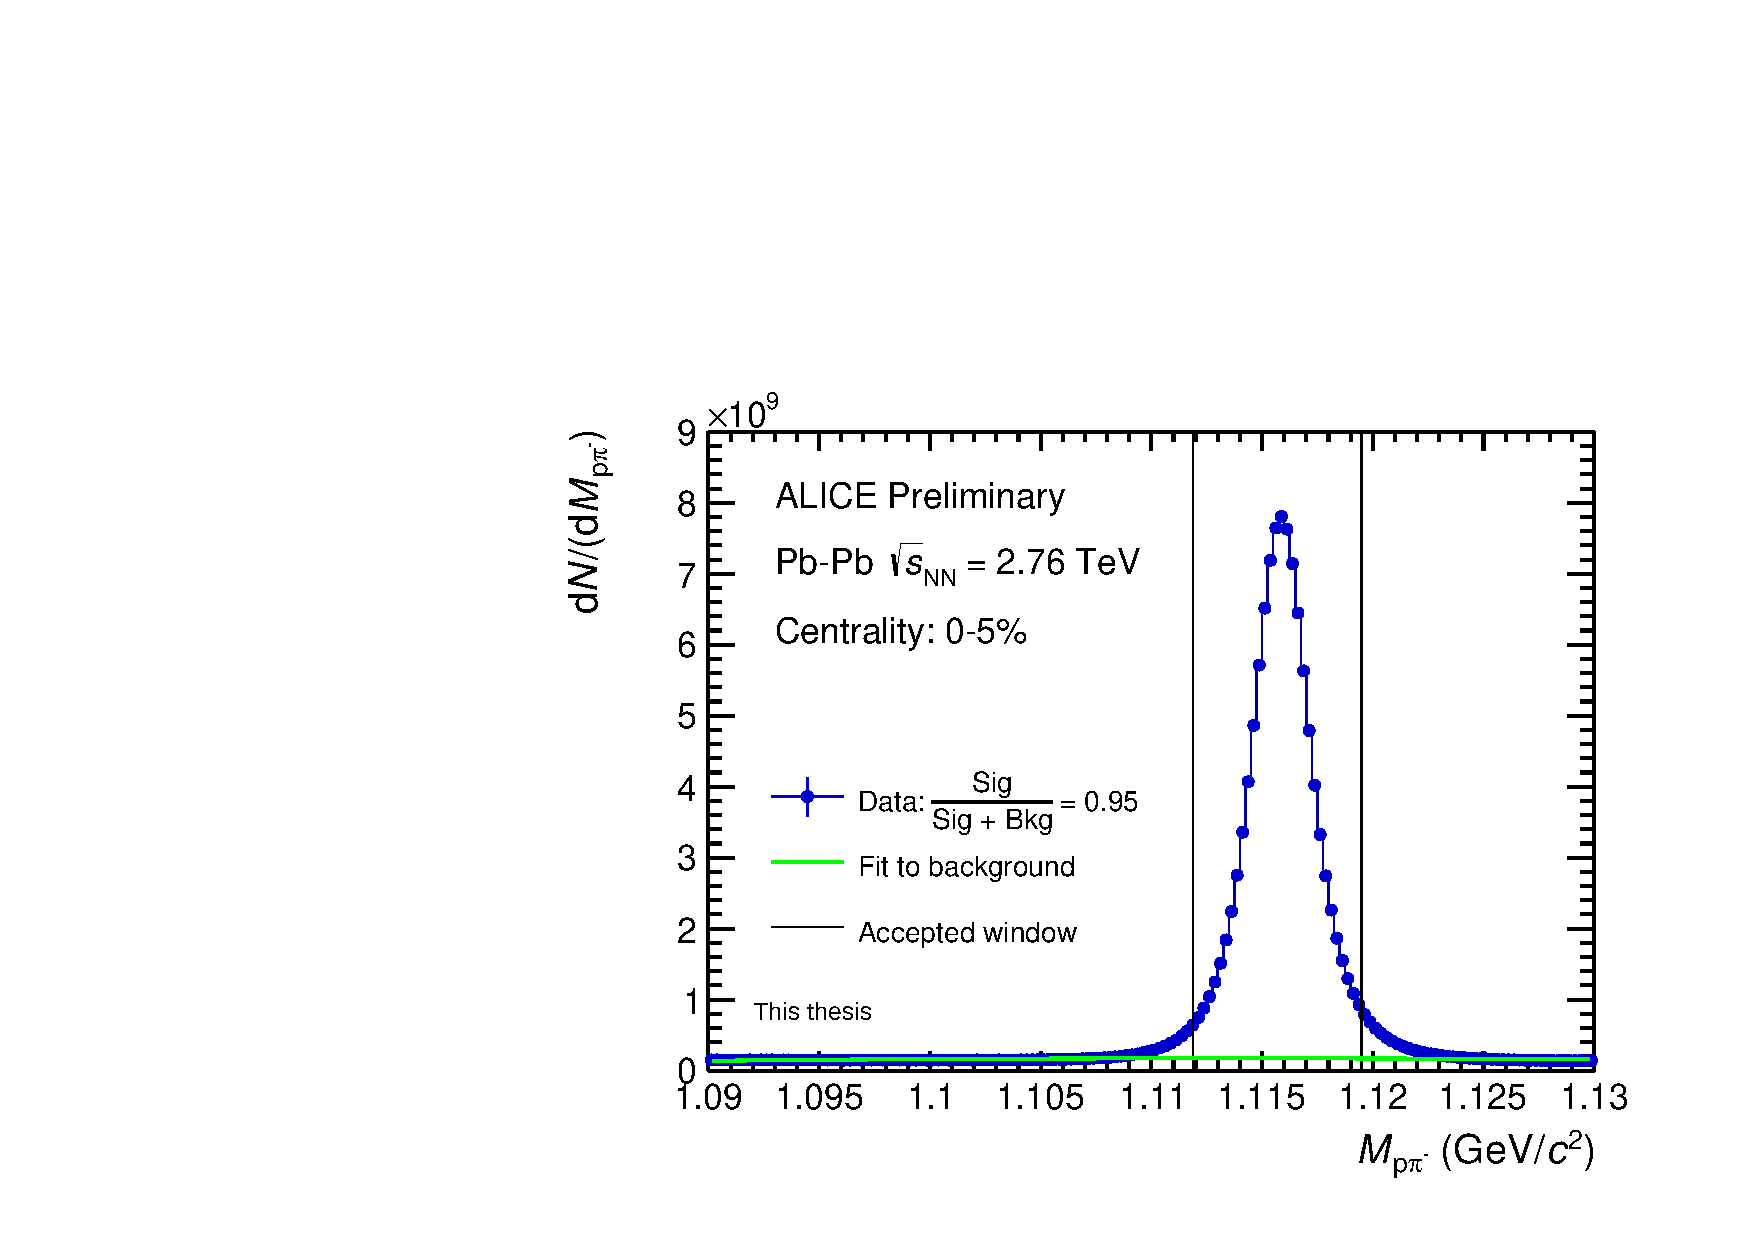
\includegraphics[width=36pc]{Figures/2014-05-11-LamMinv-CommentCorrections.pdf}
\caption[$\Lambda$ invariant mass distribution]{Invariant mass distribution for reconstructed $\Lambda$ using the optimal analysis cuts.  
The plots show V0s reconstructed from centrality integrated LHC11h data.  
The green line shows a fourth order polynomial fit to the background, which is used to estimate the number of real and fake $\Lambda$.  
The estimated ratio of real $\Lambda$ to all reconstructed $\Lambda$ in the signal region ($ \lvert m_{\mathrm{inv}} - m_{\mathrm{PDG}}\rvert < 3.8$ MeV/$\rm c^2$) is approximately 0.95.}
\label{fig:LamInvMass}
\end{figure}

\begin{figure}[hbtp]
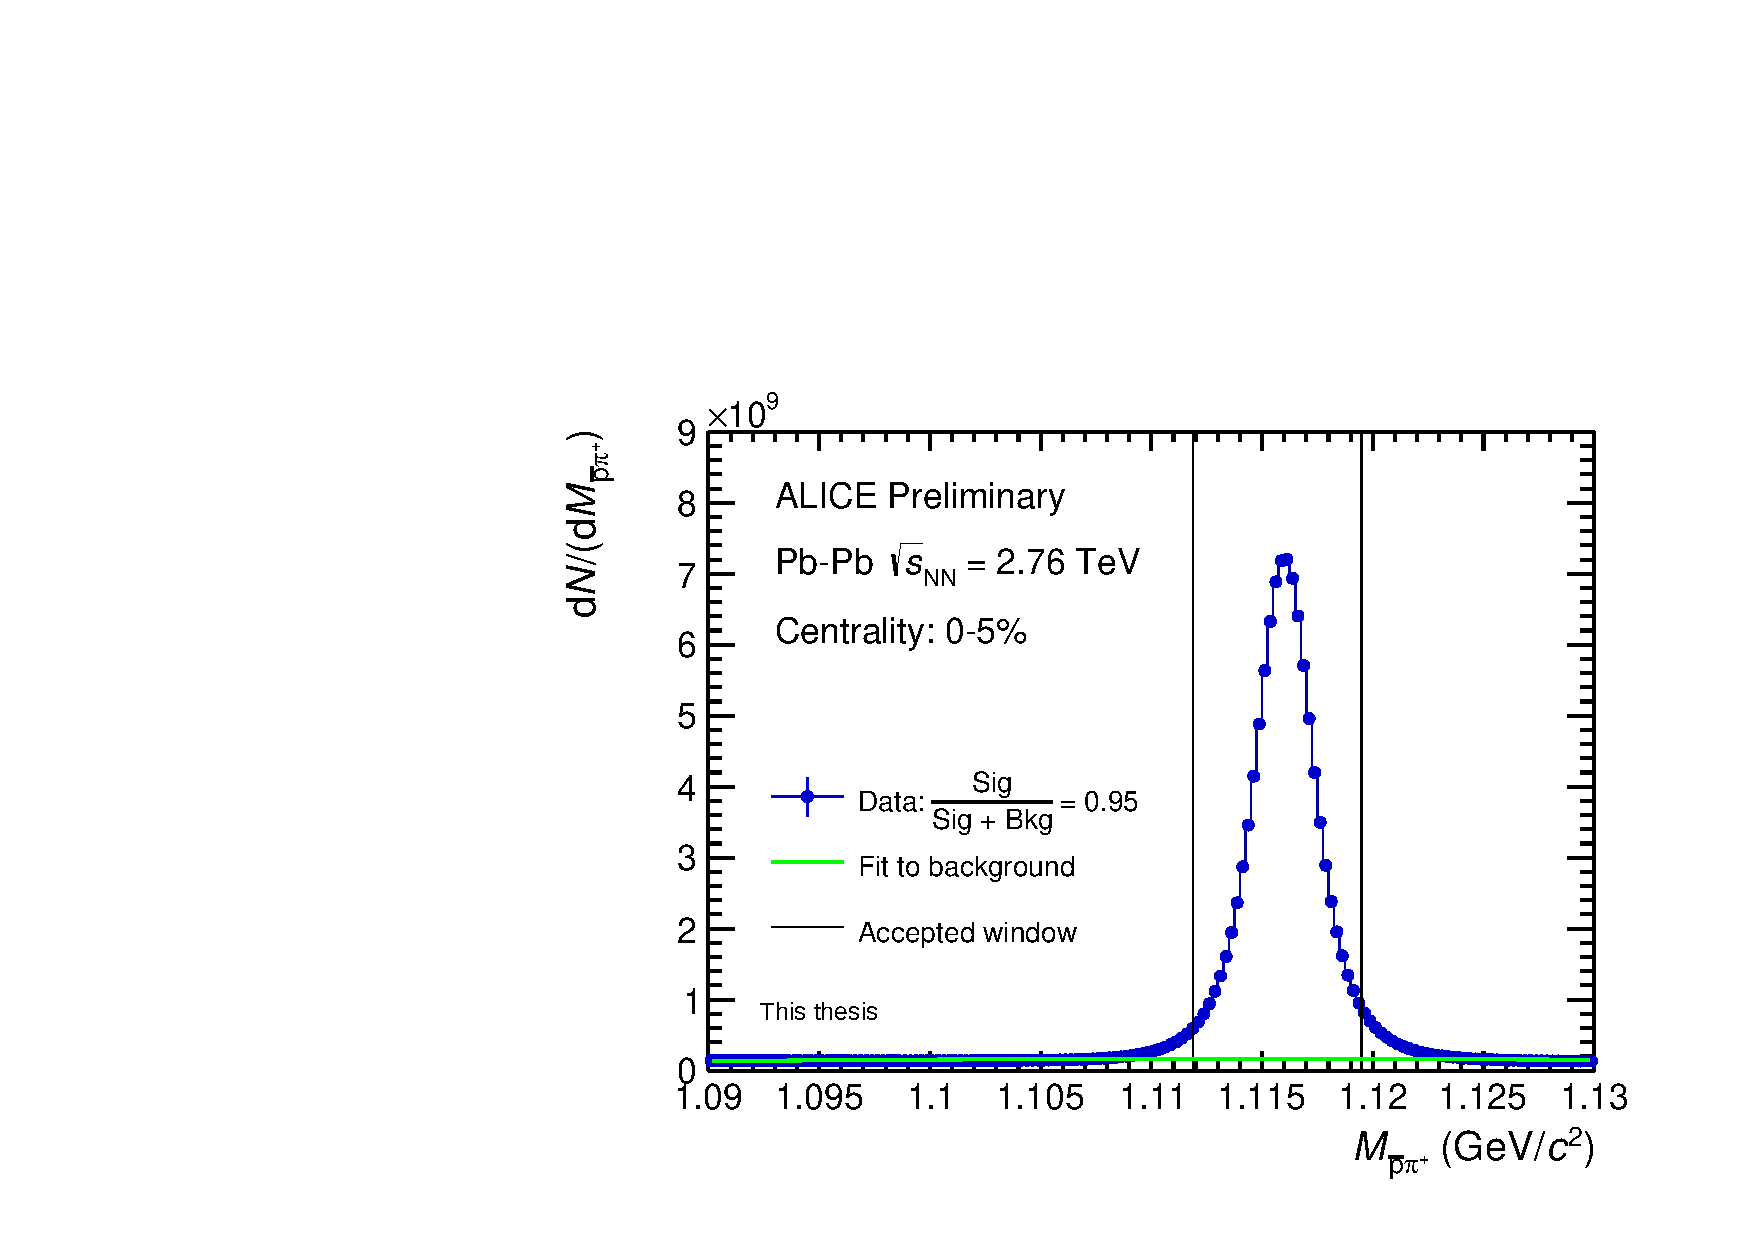
\includegraphics[width=36pc]{Figures/2014-05-11-ALamMinv-CommentCorrections.pdf}
\caption[$\bar{\Lambda}$ invariant mass distributions]{Invariant mass distribution for reconstructed $\bar{\Lambda}$ using the optimal analysis cuts.  
The plots show V0s reconstructed from centrality integrated LHC11h data.  
The green line shows a fourth order polynomial fit to the background, which is used to estimate the number of real and fake $\bar{\Lambda}$.  
The estimated ratio of real $\bar{\Lambda}$ to all reconstructed $\bar{\Lambda}$ in the signal region ($ \lvert m_{\mathrm{inv}} - m_{\mathrm{PDG}}\rvert < 3.8$ MeV/$\rm c^2$) is approximately 0.95.}
\label{fig:ALamInvMass}
\end{figure}

\subsubsection{Decay radius (XY) cut}
The V0 finder includes a default decay radius cut of 0.9 cm, which removes V0s with a radial decay length less than that value.  
This helps mitigate issues such as high track density which can complicate reconstruction.  
This analysis currently only uses the default cut, though it is possible that a tighter cut could yield improved $\Lambda$ purity without severely impacting the available statistics.  
The default cut will continue to be employed for now, but alternate cut values will be investigated in the future.  

Changes in this cut are expected to have only small effects on the correlation functions themselves.  
As will be described later in this note, fits of correlation functions have a $\lambda$ parameter which accounts for the pair-purity (roughly the square of the single particle purity).  
In any case, a few percent increase in purity should not drastically impact the shape of the correlation functions.


\subsubsection{Shared daughter cut}

Occasionally two or more V0s are reconstructed that both claim the same daughter track.  
However, a given track can only be the daughter of, at most, one V0.  
Therefore, if several reconstructed V0s all lay claim to the same daughter, at most only one of them can be a true V0.  
It was decided to employ a cut that would compare characteristics of the different V0s to determine which of them was most likely to be the true parent particle.  
After the best V0 was found, the competing V0s were removed from the list of V0 particles and not used during same- or mixed-event pair construction.

A study was done using MC event truths to determine which cut would be most successful at removing fraudulent V0s.  
The following characteristics were examined as candidates for the cut criterion:

\begin{itemize}
\item Closeness of invariant mass to the PDG mass value.
\item DCA of the daughter particles to each other.
\item Cosine of the pointing angle.
\item DCA of the V0 to the primary vertex.
\end{itemize}

The process of culling V0s with shared-daughters was done by looping through V0s on an event-by-event basis after the V0 reconstruction process was completed.  
For each V0 in the list of successfully reconstructed V0s (i.e. V0s that passed all cuts), the V0 was compared with each other V0 in the event to determine if they shared a daughter.  
Two V0s "share" a daughter if both V0s have a charged daughter track with the same track ID.  
When two V0s were found that shared a daughter, their values of the cut criterion were compared.  
The daughter with the stricter value (e.g. smaller DCA to primary vertex) was adjudged to be the better V0 candidate, and the other V0 was flagged as "bad" for failing the shared-daughter cut.  
V0s that failed the shared-daughter cut were not used in any pair construction (same event or mixed event).

However, it is possible for a V0 to share a daughter or daughters with two different V0s. 
In the aforementioned scheme, it is therefore possible for an excessive number of V0s to fail the shared daughter cut (excessive in that some of those failed V0s only shared a daughter with another failed V0).  
To avoid throwing away too many V0s, a second loop was added to shared-daughter cut method to un-flag V0s that no longer share a daughter with any "good" V0. 
Example: V0s "A" and "B" both share a daughter, and V0s "A" and "C" share a different daughter.  "A" has a better DCA than "B", so "B" is flagged as bad.  
Then "C" is found to have a better DCA than "A", so "A" is flagged as bad.  
Finally, "B" is re-flagged as good because it no longer shares a daughter with any other good V0.

This method was adapted to run iteratively over the list of V0s candidates until a stable list of non-sharing V0s was found.  
Then the MC truths of each V0 (those marked "good" and those marked "bad") were examined.  
With this information, it is possible to calculate the percentages of true V0s and fake V0s that are removed via this process.  
This analysis was run several times, each time using a different comparison criterion from the list above.

Based on the MC truth study, keeping the V0 with the closest DCA to the primary vertex was found to successfully keep 87\% of true V0s that had shared daughters.  
In comparison, the cosine of pointing angle criteria was also successful 87\% of the time (cos$(\Theta_\mathrm{p})$ and DCA to primary vertex are strongly correlated), the DCA of daughters to each other criteria was successful 81\% of the time, and the absolute value of mass difference criteria was successful 79\% of the time.
Based on these results, the DCA to primary vertex criteria was selected to used for the shared-daughter cut before correlation function construction.

%On average there were two competing particles per every ... events in the MC study.  When applied to analysis of the LHC11h data, the rate was two per ....

One of the benefits of this cut is that it helps remove a splitting-like effect (see Section \ref{sec:PairWiseCuts} for more on splitting), wherein a true V0 shares each of its daughters with two separate fake V0s.  
By the nature of the reconstruction cuts, all three of the V0s will be close in momentum space.  
Therefore a pair constructed from the two fake V0s will contaminate the low relative-momentum region of the correlation function.  
That pair of fake V0s does not share any daughters with each other, so it is not kept out of the correlation function by simple daughter ID checks.  
But iterative daughter-sharing cut described above is capable removing this fraudulent pair, since either of the fake V0s is likely to be removed for sharing a daughter with the true V0.


\subsubsection{Correlation function construction and pair cuts}
\label{sec:CFconstruct}

This analysis studies two-particle correlations as a function of the one dimensional relative momentum $k^*=\frac{1}{2}q_{\mathrm{inv}}=\frac{1}{2}\abs{P(m^2_1-m^2_2)/P^2 - q}$, where $P$ and $q$ are the four-vector momentum sum and difference, respectively, and $m_1$ and $m_2$ are the masses of the two particles.  
The correlation function is constructed as $C(k^*) = A(k^*)/B(k^*)$, where $A(k^*)$ is the two-particle distribution of the given event and $B(k^*)$ is the distribution of a reference event.  
In practice, the signal event histogram $A(k^*)$ is constructed by binning the $k^*$ value of each pair of particles in a single event, and repeating this for each event.  
The reference (or background) histogram is constructed by binning $k^*$ for pairs of particles taken from different events.  
Care is taken to ensure that pairs are mixed from events with similar centralities (bin width of 5\%) and primary vertex z-position (2 cm bin width).  
There are five mixed events for each real event.  
When constructing pairs of V0s from the same event, the V0s are not allowed to share a daughter with the same track id. 
The correlation functions are normalized to unity in the $ 0.3 < k^* < 0.5$ GeV/c range.

\subsubsection{Pair-wise cuts}
\label{sec:PairWiseCuts}

Femtoscopic studies look at the relative momentum of particles, and often the most interesting physics lies at very low relative momentum (around 0.1 GeV/c and lower).  
As a result, two-track reconstruction effects such as track splitting and track merging, both of which occur for tracks with similar momenta and trajectories, can have a large effect on the final results.  
Track splitting means that the track left by a single charged particle is reconstructed as two separate tracks. 
Track merging is when the tracks of two separate particles are reconstructed as a single track.  
For V0s, splitting/merging occurs on the level of the daughter tracks, and it affects the reconstruction of the parent V0s.

In this analysis, two-track reconstruction effects are combated via a cut on the average separation of daughter tracks from different lambdas.  
The average separation distance of two daughter tracks are computed at nine different radii of the TPC.  
The tracks are propagated iteratively using their local coordinates and the PropagateTo function, and their global positions are determined at 85, 105, 125, 145, 165, 185, 205, 225, and 245 cm.  
Initial iteration is performed in 1 cm steps, though a secondary propagation is done in 0.1 cm steps for better precision.  
Same- and mixed-event pairs are binned according to this separation distance.  
To obtain an estimate of the merging/splitting effects both distributions are then scaled by the number of pairs at high average separation distance (10+ cm), and a correlation function (same event pairs/ mixed event pairs) is created. 

To ensure that average separation distributions of mixed-event pairs are comparable to the same-event distributions, it is necessary to perform a shifting of the primary vertex for mixed events.  
Doing so allows the track separations to be calculated as though both events had the same primary vertex.  
Without this correction, the mixed-event distributions are biased by differences in the primary vertex location.  
One could imagine an extreme example of this if one used a 20 cm wide z-vertex bin.  
In that case, tracks from different events could be shifted relative to each other by as much as 20 cm.  
For this analysis with 2 cm z-vertex binning, and the uncorrected average separation correlation is shown in Figure \ref{fig:TwoTrackPerf} (left panel).  
In contrast, the right panel of Figure \ref{fig:TwoTrackPerf} shows the primary-vertex corrected correlation.  
To get a clear account of the difference between the two, we can look at Figure \ref{fig:TwoTrackRatio}, which shows the ratio of the corrected to uncorrected correlations.  
The ratio is above unity from between 0 and 4cm.  
We can interpret this to mean that the vertex-corrected distribution has more splitting and less merging than we would expect from the uncorrected plot.

Looking at Figure \ref{fig:TwoTrackPerf}, one can see that splitting effects are relevant out to about 1 cm, as evidenced by a relative abundance of same-event pairs.  
Merging is visible out to about 3 cm, as evidenced by a dearth of same-event pairs in that range.  
To address these effects, both same- and mixed-event V0 pairs are cut if they have a like-sign daughter pair with average separation less than 3 cm.  

However, one must be somewhat cautious here, since there are physics reasons to expect that $\Lambda\Lambda$ and $\Lambda\bar{\Lambda}$ should be suppressed at low relative momentum.  
Some of that natural, physics-driven suppression may show up as a suppression in the average separation plots of the daughter tracks.  

One alternative/complement to using an average separation cut would be to enforce a relative decay length cut, where V0s are not paired with each other if their difference between their lab frame decay length values is less than some cut value (e.g. a few cm).  
One advantage of this cut is that the decay lengths of the various particles should be independent of physics effects - i.e. independent of any quantum interference or final state interaction that might occur between the particles.  
Meanwhile, the decay length cut may minimize daughter splitting effects, as well as some merging of low- and mid-$p_{\mathrm{T}}$ daughters.  
High-$p_{\mathrm{T}}$ daughters may still be affected by merging, since higher-$p_{\mathrm{T}}$ particles have straighter trajectories in the TPC.  
An analysis of relative decay length has not been performed yet, but it may prove a useful to combat splitting/merging effects.


%  In contrast, the average separation cut likely cuts out not only splitting/merging, but also some pairs with legitimate physics affects, since particles with low average separation are also close in relative momentum.  
%In the V0 case, neutral particles whose daughters are nearly collinear (i.e. small average separation) are themselves


%\begin{figure}[hbtp]
\begin{figure}[h]
\begin{minipage}{18pc}
%\includegraphics[scale=0.6]{Figures/2013-09-15-TwoTrackPerfUncorrected.pdf}
\includegraphics[width=18pc]{Figures/2013-09-15-TwoTrackPerfUncorrected.pdf}
\end{minipage}\hspace{2pc}
\begin{minipage}{18pc}
\includegraphics[width=18pc]{Figures/2013-09-15-TwoTrackPerfCorrected.pdf}
\end{minipage} 
\caption[Two-track reconstruction effects]{\label{fig:TwoTrackPerf}Correlation function versus average separation distance in the TPC for proton daughters.  
Constructed using same-event pairs over uncorrected mixed-event pairs.  
Both splitting (enhancement) and merging (suppression) effects are visible. 
The left panel shows the distribution with uncorrected mixed-event pairs, while the right panel shows the distributions with proper primary vertex correction treatment.}
\end{figure}

\begin{figure}[hbtp]
\includegraphics[width=18pc]{Figures/2013-09-15-TwoTrackRatio.pdf}
\caption[Ratio of corrected/uncorrected average-separation distributions]{Ratio of vertex-corrected average separation plot to uncorrected average separation plot.  
The enhancement above unity at low average-separation suggests that the uncorrected distribution underestimates the amount of splitting and overestimates the amount of merging. 
The differences between the plots seems to disappear (i.e. ratio goes to unity at $\approx$ 3 cm.}
\label{fig:TwoTrackRatio}
\end{figure}

\subsubsection{Momentum resolution correction}
\label{sec:MomentumResCorrectionCF}

There is an inherent resolution to V0 momenta that depends on the resolution of the reconstructed daughter tracks.  
Because of this limit of precision, there is also an associated resolution to the relative momentum of two V0s.
This causes the reconstructed relative momentum of the pair to differ from the true momentum of the pair, and it therefore introduces subtle changes to the measured correlation functions which must be accounted for.

Tradionally, the momentum resolution correction is performed on the experimental data to unsmear it into a form that should resemble the theoretical predictions (i.e.\ fits). 
In this analysis we have instead chosen to smear the fits to conform to the experimental data. 
The experimental correlation functions therefore remain uncorrected. 
As our corrections are employed at the time of fitting, we'll discuss the full methodology in section \ref{sec:MomResCorrectFit}.